\documentclass[review,12pt,authoryear]{elsarticle}

\usepackage{graphicx}
% Editorial Manager flattens uploads into one folder; keep ./ first so the
% portal finds bare figure names. Local builds resolve files under ../figures/.
\graphicspath{{./}{../figures/}{figures/}}
\usepackage{epstopdf}
\usepackage{booktabs}
\usepackage{amsmath,amssymb}
\usepackage{textcomp}
\usepackage{url}
\makeatletter
\g@addto@macro{\UrlBreaks}{\do\-\do\_\do\.\do\+\do\=\do\@}
\makeatother
\usepackage[table]{xcolor}
\usepackage{float}
\usepackage{placeins}

\journal{Toxicology}

\begin{document}

\begin{frontmatter}

\title{Directional transfer of chemical-gene effects from rodents to humans:
an independence-guarded meta-analysis of the Comparative Toxicogenomics
Database}

% Double-blind review: author names, affiliations and the corresponding-author
% email are intentionally omitted from this manuscript and are provided on the
% separate title page.
\author{}

\begin{abstract}
Animal-to-human extrapolation is the central validity problem in toxicology,
yet the reliability with which a chemical's directional effect on a gene
transfers across species has not been quantified at scale. Using the
Comparative Toxicogenomics Database, we assembled 1{,}165{,}406 curated
chemical-gene-endpoint effects across human, mouse and rat and asked how often
a rodent directional call (increases or decreases) matches the human call. The
evidence base is curated in vivo and in vitro findings; exposure doses and
durations are not standardized across the source literature, so the estimand is
literature-level directional concordance rather than controlled biological
replication. Because a naive comparison is circular when both calls come from
the same publication, the primary analysis was restricted to 40{,}779 effects
with disjoint PubMed identifiers across species. Independent directional
agreement was 62.0\% (95\% CI 61.5-62.5), only 11.4 points above chance and
close to the 66.2\% mouse-versus-rat within-rodent benchmark; human-specific
divergence was 4.2 points (95\% CI $-$1.1 to 10.9). Shared-publication
co-curation inflated agreement to 89.2\%. Transfer varied more by molecular
endpoint (activity 89\%, expression 61\%, methylation at chance) and replication
depth (61\% at one report per species, rising to 100\% at five) than by chemical
class (variance component $\approx$1\%), localising to the specific
chemical-gene pair (intraclass correlation 0.44). Transfer was weakly
predictable for unseen chemicals (grouped cross-validated AUC 0.58), and
human-rodent protein identity was not associated with transfer (odds ratio 0.97
per 10 points, 95\% CI 0.94-1.00). Cross-species directional disagreement is
largely generic and context-dependent rather than tracking evolutionary
distance.
\end{abstract}

\begin{keyword}
toxicogenomics \sep cross-species extrapolation \sep new approach methodologies
\sep reproducibility \sep Comparative Toxicogenomics Database \sep ortholog
conservation
\end{keyword}

\end{frontmatter}

%=========================================================================
\section{Introduction}
%=========================================================================

Almost everything we believe about how chemicals perturb human biology is
inferred, at some remove, from rodents. That inference is the foundation of
regulatory toxicology and of preclinical drug development, and it is also their
best-documented weakness: across large bodies of comparisons, animal results
translate to humans with wide and often disappointing concordance
\citep{leenaars2019,marshall2023}, big safety databases confirm that animal
findings are informative but far from sufficient predictors of human toxicity
\citep{clark2018,liu2026}, and even at the level of the transcriptome the
concordance between species has been contested strongly enough to support
opposite published conclusions from the same data \citep{seok2013,takao2015}. The
response from regulators and funders has been to re-weight the evidence base:
from the founding principles of replacement, reduction and refinement
\citep{russell1959} to the current pivot toward human-relevant new approach
methodologies and the regulatory acceptance of non-animal evidence in drug
submissions \citep{wu2026science}. All of this presupposes an answer to a
question that has never been quantified at the level of individual molecular
effects: \emph{when a chemical moves a gene in a given direction in a rodent, how
often does the same directional effect hold in a human?}

Individual studies have compared species for one chemical or one organ, but a
comprehensive, effect-level answer requires a resource that has already
harmonised the vocabulary of chemical action across species and the literature.
The Comparative Toxicogenomics Database (CTD) is that resource: a manually
curated compendium of chemical-gene, chemical-disease and gene-disease
relationships drawn from the published literature, in which each chemical-gene
interaction carries a signed action (for example, ``increases expression'' or
``decreases activity''), an organism, and its supporting references
\citep{mattingly2003ctd,davis2025ctd}. This makes it possible to line up, for a
given chemical, gene and molecular endpoint, the directional call curated in
humans against the call curated in rodents, across tens of thousands of
independent instances.

The apparently obvious analysis, simply asking how often the human and rodent
calls agree, is fatally circular. A large fraction of cross-species pairs are
curated from the \emph{same} publications: a single paper that reports an effect
in both a human cell line and a mouse contributes a matched pair whose agreement
is guaranteed by construction and reflects the curation pipeline rather than
biology. Any honest estimate must therefore isolate the pairs whose human and
rodent evidence come from disjoint references. This distinction between
apparent and independent concordance is, to our knowledge, absent from prior
cross-species toxicogenomic work, and it turns out to matter enormously.

We report an independence-guarded meta-analysis of directional transfer in CTD.
We pre-specified four aims: (i) to estimate independent human-rodent directional
agreement overall and stratified by molecular endpoint, chemical class and
replication depth, benchmarked against a within-rodent (mouse-versus-rat)
agreement benchmark; (ii) to decompose non-agreement into within-species
inconsistency and genuine between-species divergence; (iii) to test whether
transfer is predictable for chemicals never seen in training, using
grouped cross-validation; and (iv) to test, against a pre-registered anchor
lying entirely outside CTD curation, whether evolutionary conservation of the
gene explains transfer. Framing throughout is deliberately descriptive: the
substrate is curated published findings, and the estimands are conditional on
curation.

%=========================================================================
\section{Materials and methods}
%=========================================================================

\subsection{Data source and release}

We used the CTD bulk data files (release of 30 July 2026), comprising the
curated chemical-gene interaction file and the chemical, gene and pathway
vocabularies \citep{davis2025ctd}. The external conservation anchor was built
from NCBI \texttt{gene\_orthologs} and Ensembl Compara, both independent of CTD
\citep{brown2015ncbigene,austine2025ensembl}.
All definitions below were fixed in a configuration file before analysis, and
the full pipeline is deterministic given a fixed random seed.

\subsection{Experimental system and human relevance}

The experimental systems underlying this study are the curated in vivo (human,
mouse and rat) and in vitro chemical-gene findings recorded in CTD; the analysis
operates on directional calls abstracted from many thousands of primary studies
rather than on a single controlled exposure. Human relevance is intrinsic to the
design rather than extrapolated: the primary estimand compares each rodent
directional effect with the \emph{directly curated human} directional effect for
the same chemical and gene, so the human comparator is measured, not inferred
from a model species. Because the substrate is aggregated curated literature, the
exposure dose or concentration and duration, and the CAS number, source and
purity of each chemical, are properties of the individual source experiments and
are neither standardized nor controllable at the level of this meta-analysis; we
therefore treat them as uncontrolled and report agreement conditional on
curation, and we do not draw dose- or purity-dependent conclusions. Randomization
of treatment groups does not apply to a retrospective curated census; in its
place, unit-level replication is the number of independent supporting
publications per species (the replication-depth stratification of
Section~\ref{sec:results}), and all inferential procedures (Wilson intervals,
chemical-cluster bootstraps and grouped cross-validation) are specified below.

\subsection{Effect keys and directional consensus}

The unit of analysis is an \emph{effect key}: a (chemical, gene, molecular
endpoint) triple. We retained single-action, signed interactions whose action
carried an interpretable direction, that is, ``increases'' or ``decreases''
applied to one of the molecular endpoints expression, activity, methylation,
phosphorylation, secretion, abundance, cleavage, metabolic processing,
stability, uptake, transport and related aspects; multi-action and unsigned
interactions were excluded. Records were grouped into three species by NCBI
taxonomy identifier: human (9606), mouse (10090) and rat (10116); mouse and rat
were pooled as ``rodent'' for the primary contrast and analysed separately for
the within-rodent (mouse-versus-rat) benchmark.

For each effect key and species we counted ``increases'' and ``decreases''
curations and assigned a consensus direction: $+1$ if only increases were
curated, $-1$ if only decreases, and $0$ (ambiguous) if both directions or none
appeared. We also recorded, per species, the set of supporting PubMed
identifiers. The analytic table contained 1{,}165{,}406 effect keys.

Two points about interpretation follow from this construction, and we return to
them throughout. First, a matched human and rodent call need not derive from the
same tissue, dose, exposure duration or cell type; what we measure is therefore
the concordance of curated directional calls across the literature, which is a
necessary condition for biological reproducibility but is not a controlled
biological replication of it. Second, every estimand is conditional on what has
been published and curated, and inherits the corresponding selection. We use
``agreement'' and ``transfer'' throughout as shorthand for this literature-level
directional concordance, not as a direct claim about biological reproducibility.

\subsection{Independence guard}

For every key measured in both human and rodent we computed the intersection of
their supporting PubMed identifiers. A pair was \emph{independent} (PMID-disjoint)
if that intersection was empty, so that the human and rodent directional calls
rest on non-overlapping primary literature. The primary population comprised
keys measured in both species, with an unambiguous consensus in each, and with
disjoint supporting references. Keys sharing at least one reference were analysed
separately to quantify co-curation inflation.

\subsection{Aim 1: reproducibility}

The primary estimand was the probability that the human consensus direction
equals the rodent consensus direction, among independent unambiguous pairs. We
report the point estimate with a Wilson interval \citep{wilson1927} and, because
keys are nested within chemicals and genes, a cluster (block) bootstrap with
chemicals as the resampled unit and 1{,}000 replications \citep{davison1997boot}.
A chance-agreement baseline was computed from the marginal direction
frequencies in each stratum. Mouse-versus-rat agreement, estimated identically,
provided a within-rodent benchmark: an upper reference for the agreement
attainable between two closely related mammals studied through the same curated
literature. This benchmark is not a pure reproducibility floor, because mouse and
rat are distinct species with genuine biological differences; it bounds the
combination of curation reproducibility and closely-related-species divergence.
Because it already absorbs some true biological divergence, any excess
disagreement for human-versus-rodent over this benchmark is a conservative
estimate of the specifically human-versus-rodent component.
Pre-specified strata were molecular endpoint, coarse chemical class from the
MeSH chemical tree, and replication depth (the minimum number of supporting
references on either side).

\subsection{Aim 2: decomposition}

Non-agreement can arise two ways: a species may be internally inconsistent (the
same key curated both up and down within one species, reflecting context, time
or tissue dependence, or curation noise), or each species may be internally
consistent yet disagree with the other. We measured within-species
inconsistency as the fraction of multiply-curated keys that were internally
ambiguous, separately in each species. We defined human-specific divergence as
the difference between human-versus-rodent disagreement and the mouse-versus-rat
benchmark, with a cluster bootstrap interval; a value near zero indicates that
cross-species disagreement is already present within a single clade rather than
being a specifically human-versus-rodent phenomenon. Finally, we partitioned the variance of the
binary agreement outcome across grouping factors (chemical, gene, endpoint,
chemical class, and the chemical-gene pair) using a one-way intraclass
correlation coefficient \citep{shrout1979icc}, which estimates the share of
agreement variance attributable to each factor.

\subsection{Aim 3: predictability}

We asked whether, given only rodent-side information, the human direction is
predictable for a chemical never seen during training. The outcome was
agreement (human direction equal to rodent direction) on the independent
unambiguous set. Features were known at prediction time and used no human-side
information: molecular endpoint, chemical class, rodent consensus direction,
rodent evidence depth and support, and chemical and gene promiscuity (the number
of distinct keys involving each) and gene pathway membership. We fitted a
regularised logistic model and a histogram gradient-boosting classifier
\citep{friedman2001gbm,ke2017lightgbm,pedregosa2011sklearn} under
\emph{grouped} five-fold cross-validation with chemicals as groups, so that no
chemical appeared in both training and test folds; this prevents the optimistic
leakage that ordinary cross-validation would introduce through repeated
chemicals \citep{kaufman2012leakage}. We report discrimination (area under the
ROC curve, average precision), calibration (reliability curve, Brier score) and
model-agnostic permutation importance, together with a leave-one-chemical-class-out
generalisation test.

\subsection{Aim 4: external conservation anchor}

Every quantity above is internal to CTD curation. To test whether the result is
self-referential, we pre-registered, before any Aim 4 modelling, a single
external anchor: evolutionary conservation of the human gene to its rodent
ortholog, taken from sources outside CTD. Graded conservation was the protein
percent identity of the human gene to its mouse and rat orthologs from Ensembl
Compara (we used the per-gene mean and minimum across the two rodents)
\citep{austine2025ensembl}; orthology status was the one-to-one flag from
Ensembl, with the NCBI \texttt{gene\_orthologs} one-to-one flag as a secondary
anchor \citep{brown2015ncbigene}. The directional, pre-specified hypothesis was
that transfer increases with conservation: if cross-species failure were driven
by molecular divergence, effects on highly conserved genes should transfer more
reliably. We related agreement to conservation quartile with cluster-bootstrap
intervals, estimated a chemical-cluster-robust logistic trend (odds ratio per 10
percentage points of identity), contrasted one-to-one against other orthology,
and tested whether conservation adds discrimination to the Aim 3 model under the
same grouped cross-validation. The relevance of orthology conjecture debates to
functional transfer motivated this design \citep{nehrt2011,chen2012ortholog}.

\subsection{Software and reproducibility}

Analyses used Python with pandas, NumPy, SciPy, statsmodels and scikit-learn
\citep{pedregosa2011sklearn}. Cluster-robust inference used chemical as the
clustering unit throughout. Code and non-identifiable aggregate tables are
openly available at
\url{https://github.com/january-msemakweli/Cross-Species-Directional-Transfer-Chemical-Gene-Effects}.

%=========================================================================
\section{Results}
\label{sec:results}
%=========================================================================

\subsection{Independent cross-species agreement is modest, and co-curation
inflates it}

Of 1{,}165{,}406 effect keys, 61{,}439 were curated in both a human and a rodent
context. Restricting to keys with an unambiguous consensus in each species and,
critically, to those whose human and rodent evidence came from disjoint
publications left 40{,}779 independent pairs. Among these, the human and rodent
directional calls agreed 62.0\% of the time (95\% CI 61.5-62.5; cluster
bootstrap 58.7-65.4), which is 11.4 percentage points above the 50.6\% chance
baseline (Table~\ref{tab:1}, Figure~\ref{fig:1}). When the independence guard
was removed and pairs sharing at least one reference were examined, apparent
agreement rose to 89.2\% (88.3-90.1). The gap between these two numbers is the
central methodological result: roughly two-thirds of the naive concordance one
would report from CTD without an independence guard is an artefact of the same
paper being curated into both species.

The independent estimate is best read against a within-rodent benchmark.
Mouse-versus-rat agreement, estimated identically on 25{,}615 pairs, was 66.2\%
(65.6-66.7). This is the agreement attainable between two closely related
rodents through the same curated literature; it blends curation reproducibility
with any genuine mouse-rat biological differences, and so is an upper reference
rather than a pure noise floor. Independent human-rodent agreement (62.0\%) sits
only just below it, which already reframes the problem: most of what looks like a
human-specific species barrier is present even between two rodents.

\begin{table}[H]
\centering
\caption{Directional agreement of chemical-gene effects across species. The
primary estimate is restricted to pairs whose human and rodent evidence come
from disjoint publications; the shared-publication stratum shows the inflation
that an independence guard removes; the mouse-versus-rat stratum is a
within-rodent benchmark that blends curation reproducibility with genuine
mouse-rat biological differences. Bootstrap intervals resample chemicals.}
\label{tab:1}
\setlength{\tabcolsep}{5pt}
\resizebox{\linewidth}{!}{%
\begin{tabular}{@{}lcccccc@{}}
\toprule
Comparison & Pairs (n) & Agreement & Wilson 95\% CI$^{\mathrm{a}}$ &
Bootstrap 95\% CI$^{\mathrm{b}}$ & Chance & Excess$^{\mathrm{c}}$ \\
\midrule
\textbf{Human vs rodent, independent (primary)} & 40{,}779 & \textbf{62.0\%} &
61.5-62.5 & 58.7-65.4 & 50.6\% & +11.4 \\
Human vs rodent, all pairs & 45{,}557 & 64.9\% & 64.4-65.3 & 61.7-68.4 &
50.9\% & +14.0 \\
Human vs rodent, shared publication & 4{,}778 & 89.2\% & 88.3-90.1 & 80.2-96.1 &
54.5\% & +34.8 \\
Mouse vs rat (within-rodent benchmark) & 25{,}615 & 66.2\% & 65.6-66.7 &
58.7-74.8 & 45.2\% & +21.0 \\
\bottomrule
\end{tabular}%
}

\vspace{3pt}
\begin{minipage}{\linewidth}
\scriptsize
$^{\mathrm{a}}$ Wilson score interval for the point estimate, treating pairs as
independent. \\
$^{\mathrm{b}}$ Cluster bootstrap resampling chemicals (1{,}000 replications);
wider than the Wilson interval because it propagates within-chemical
correlation. This is the interval used for all inference and shown in the
figures. \\
$^{\mathrm{c}}$ Percentage points above the stratum-specific chance baseline
derived from marginal direction frequencies.
\end{minipage}
\end{table}

\begin{figure}[H]
\centering
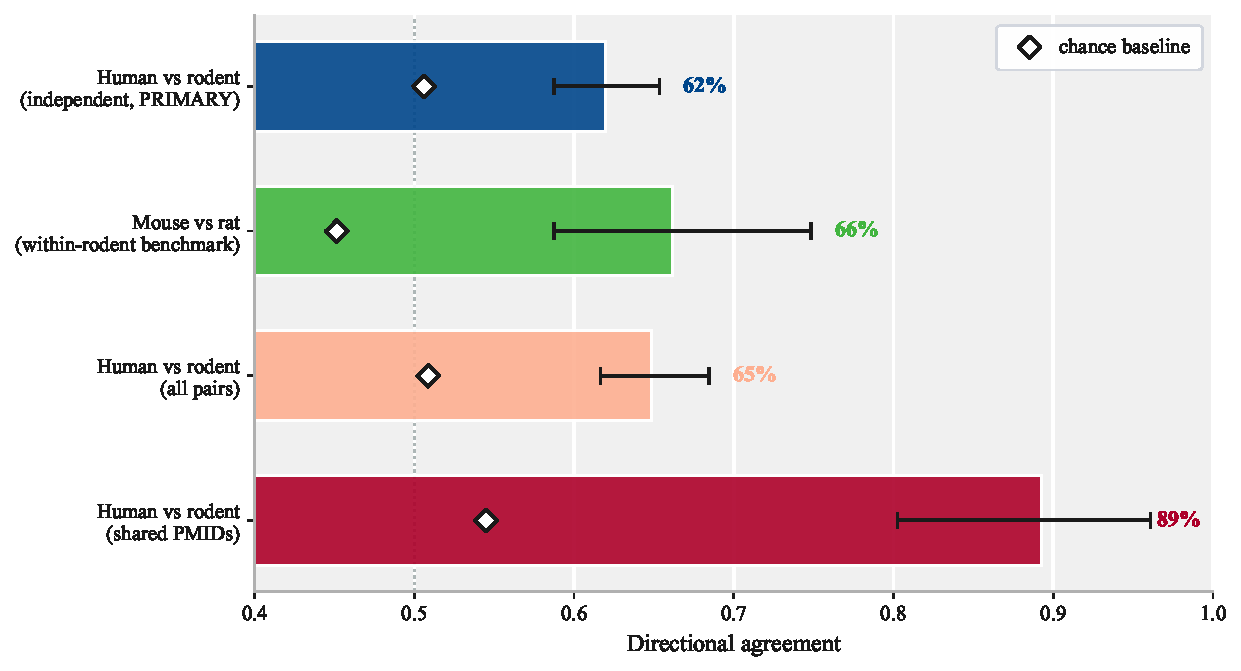
\includegraphics[width=0.86\linewidth]{F1_overview_agreement.pdf}
\caption{Directional agreement of chemical-gene effects by comparison. Bars
are point estimates with cluster-bootstrap 95\% intervals (chemicals resampled);
diamonds mark the stratum-specific chance baseline. Independent human-rodent
agreement (navy) is far below the shared-publication estimate and sits just
below the mouse-versus-rat within-rodent benchmark.}
\label{fig:1}
\end{figure}

\subsection{Transfer is governed by molecular endpoint and replication depth,
not chemical class}

Agreement was strongly heterogeneous across molecular endpoints
(Figure~\ref{fig:2}, Supplementary Table~S1). Functional endpoints transferred
well: cleavage 96.7\% (n=182), activity 89.3\% (n=1{,}106), secretion 85.7\%
(n=286) and phosphorylation 81.5\% (n=744). Bulk molecular endpoints transferred
poorly: gene expression, which dominates the data (n=36{,}986), agreed only
60.8\% of the time, and DNA methylation (n=1{,}102) agreed 41.9\%, essentially at
its 40.9\% chance baseline. A directional effect on methylation curated in a
rodent therefore carries almost no information about the direction in a human.

Replication depth was the strongest ordered signal (Figure~\ref{fig:3},
Supplementary Table~S2). Agreement rose monotonically from 60.7\% for effects
supported by a single report on the thinner side, to 76.5\% at two, 90.6\% at
three, 95.6\% at four, and 100\% at five or more supporting reports per species.
Multiply-replicated directional effects transfer nearly deterministically; the
modest headline number is a property of the long tail of singly-curated effects,
not of the well-established ones.

By contrast, chemical class barely mattered. Agreement ranged only from 59.1\%
for metals to 68.6\% for heterocyclic organics (Supplementary Table~S3), a
spread small enough that, as shown next, chemical class explains almost none of
the variance in transfer.

\begin{figure}[H]
\centering
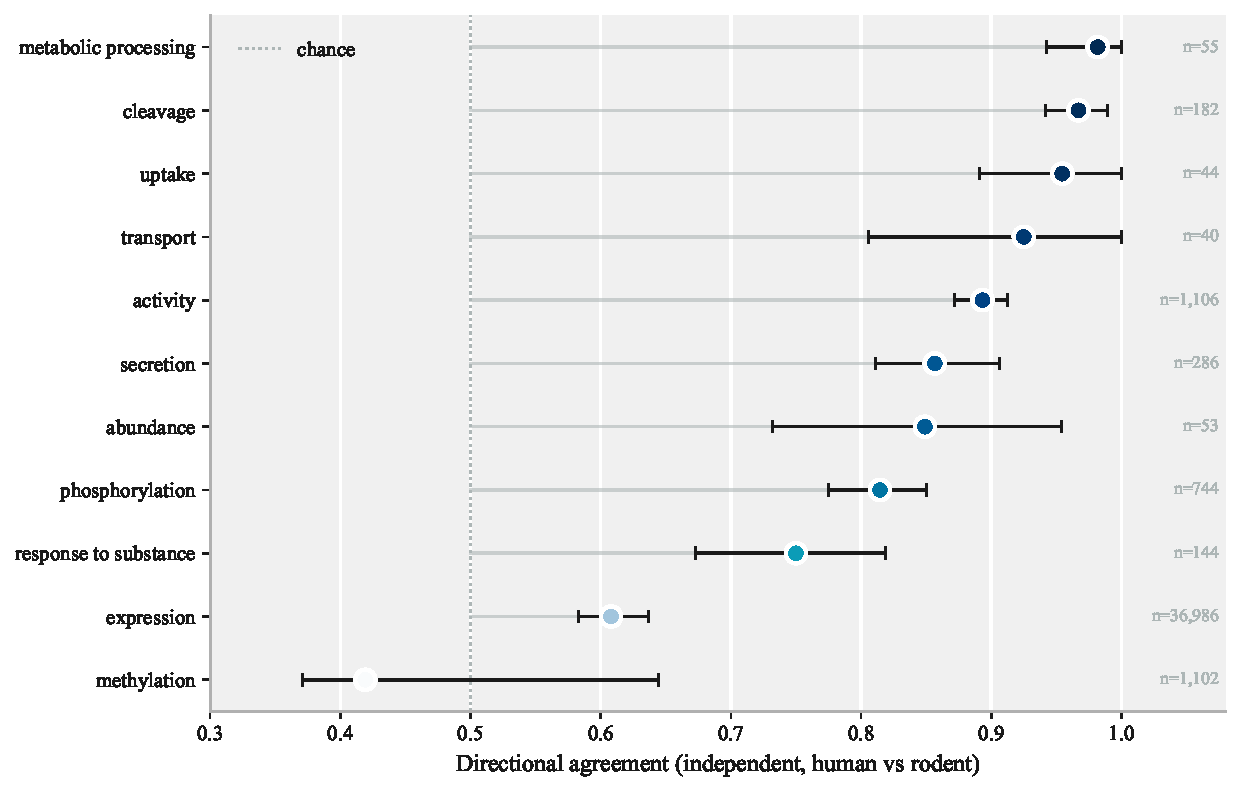
\includegraphics[width=0.80\linewidth]{F2_by_aspect.pdf}
\caption{Independent human-rodent directional agreement by molecular endpoint,
ordered by agreement, with cluster-bootstrap 95\% intervals and per-stratum
sample sizes. The dotted line marks chance. Functional endpoints (activity,
secretion, phosphorylation, cleavage) transfer well; bulk expression is modest
and methylation sits at chance.}
\label{fig:2}
\end{figure}

\begin{figure}[H]
\centering
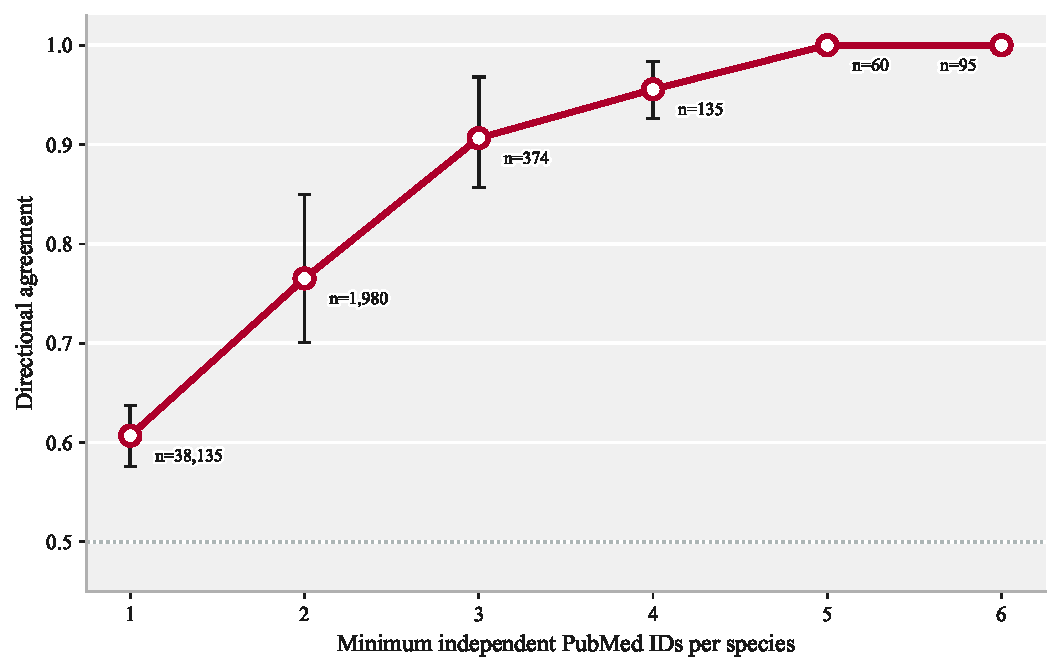
\includegraphics[width=0.70\linewidth]{F3_depth.pdf}
\caption{Independent directional agreement as a function of replication depth,
the minimum number of supporting publications per species, with
cluster-bootstrap 95\% intervals. Agreement climbs from $\sim$61\% at a single
report to 100\% at five or more.}
\label{fig:3}
\end{figure}

\subsection{Cross-species disagreement is largely generic and localises to the
chemical-gene pair}

Two analyses locate the disagreement. First, within-species inconsistency is
large: of keys curated more than once, 58.3\% were internally ambiguous in
humans, 54.5\% in mouse and 65.9\% in rat (Supplementary Table~S4). A substantial
share of apparent cross-species disagreement is simply that a single species does
not reproduce its own directional call. Second, human-specific divergence is
small: human-versus-rodent disagreement (38.0\%) exceeded the mouse-versus-rat
benchmark (33.8\%) by only 4.2 percentage points, with a cluster-bootstrap
interval that
crosses zero ($-$1.1 to 10.9; Figure~\ref{fig:4}A). The extra penalty for
crossing from rodent to human, over and above the penalty for crossing between
two rodents, is not distinguishable from zero.

The variance decomposition (Figure~\ref{fig:4}B, Supplementary Table~S5) is
consistent. The intraclass correlation of the agreement outcome was 0.44 for the
chemical-gene pair, but only 0.12 for molecular endpoint, 0.068 for gene, 0.046
for chemical and 0.005 for chemical class. Transferability is thus overwhelmingly
a property of the specific chemical-gene combination, not of broad chemical
categories: knowing the class of a chemical tells you almost nothing about
whether its effects transfer, whereas the identity of the exact pair tells you a
great deal.

\begin{figure}[H]
\centering
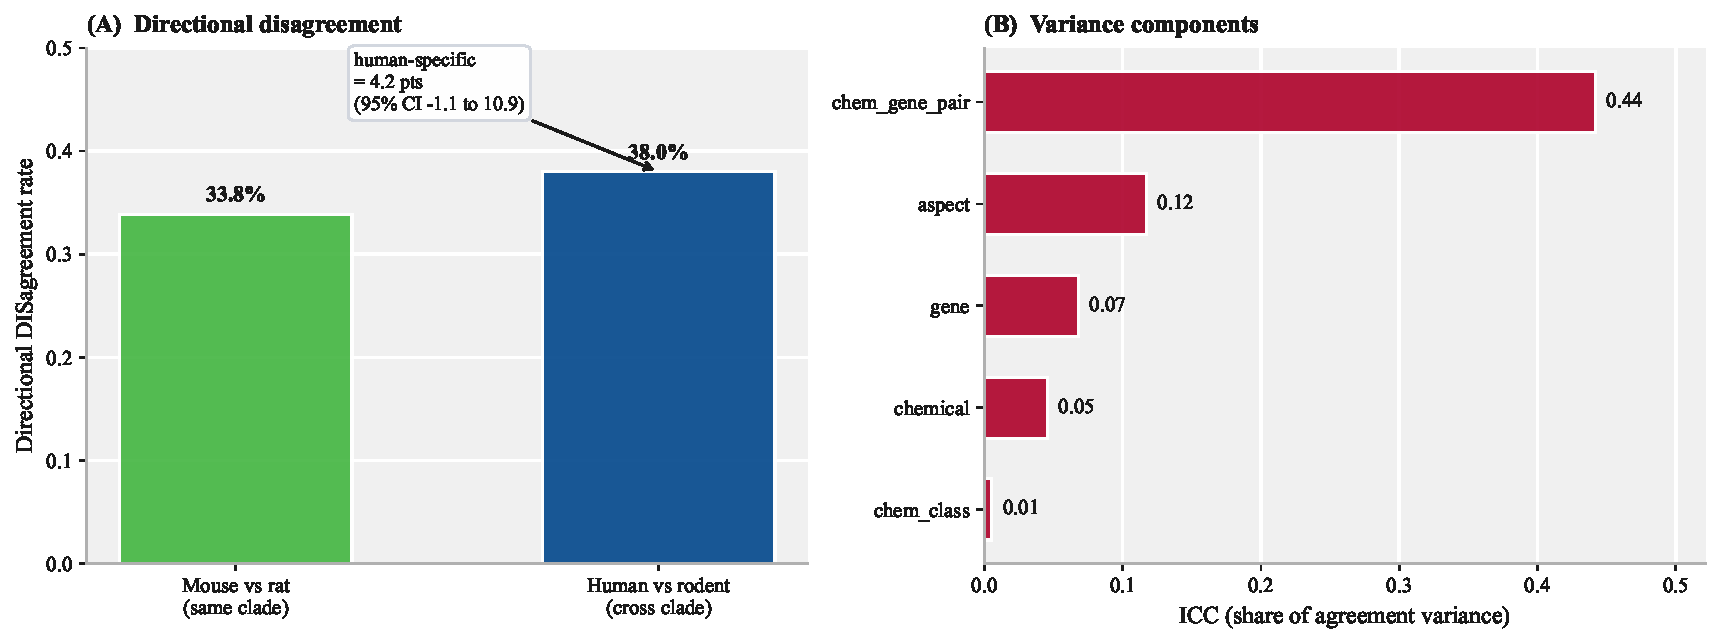
\includegraphics[width=\linewidth]{F4_decomposition.pdf}
\caption{Decomposition of non-agreement. (A) Directional disagreement between
mouse and rat (same clade) versus between human and rodent (cross clade); the
human-specific excess is 4.2 percentage points with a bootstrap interval that
includes zero. (B) Intraclass correlation of the binary agreement outcome by
grouping factor; transfer localises to the specific chemical-gene pair, not to
chemical class.}
\label{fig:4}
\end{figure}

\subsection{Transfer is only weakly predictable for unseen chemicals}

Under grouped cross-validation with chemicals held out, rodent-side features
predicted human agreement only weakly: the gradient-boosting model reached an
area under the ROC curve of 0.58 (SD 0.02 across folds) and the logistic model
0.56, against a 62\% prevalence baseline (Figure~\ref{fig:5},
Supplementary Table~S6). The model was well calibrated (Figure~\ref{fig:5}A) and
the most informative features were the rodent direction itself, gene promiscuity,
molecular endpoint and rodent evidence depth (Figure~\ref{fig:5}B); chemical
class contributed nothing, consistent with the variance decomposition.
Leave-one-chemical-class-out AUCs ranged from 0.51 to 0.61. The honest reading is
that no compact set of chemical- or gene-level covariates recovers transferability
for a genuinely new chemical; the information lives at the pair level, which is
by definition unavailable for unseen chemicals.

\begin{figure}[H]
\centering
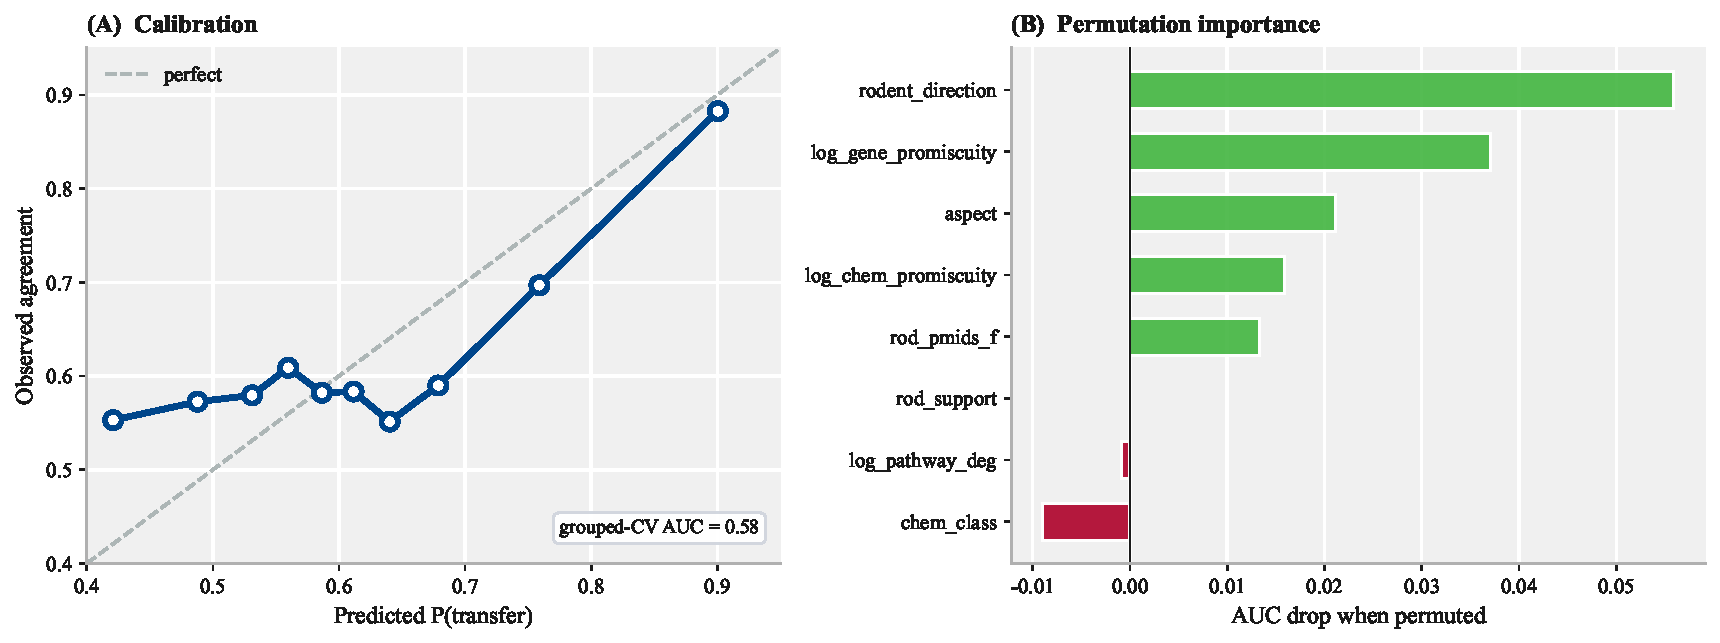
\includegraphics[width=\linewidth]{F5_prediction.pdf}
\caption{Predicting directional transfer for unseen chemicals under grouped
(by chemical) five-fold cross-validation. (A) Reliability curve for the
gradient-boosting model against the line of perfect calibration, with the
grouped cross-validated AUC. (B) Permutation importance; the rodent direction,
gene promiscuity, molecular endpoint and rodent evidence depth carry the signal,
while chemical class does not.}
\label{fig:5}
\end{figure}

\subsection{Sequence conservation is not associated with transfer}

The external anchor closes the circularity concern and returns a clean null.
Conservation coverage was near-complete: 39{,}933 of 40{,}779 primary keys
(97.9\%) had an Ensembl human-rodent identity value (median 87.5\%). Directional
agreement was flat across the entire range of conservation
(Figure~\ref{fig:6}A): 63.0\% in the least-conserved quartile (median 70\%
identity), 61.8\% and 62.9\% in the middle quartiles, and 60.5\% in the
most-conserved quartile (median 97\% identity). The chemical-cluster-robust
logistic trend was null, and if anything slightly negative: odds ratio 0.97 per
10 percentage points of identity (95\% CI 0.94-1.00, $p=0.07$). One-to-one
orthology did nothing (Ensembl odds ratio 1.02, 95\% CI 0.96-1.09; NCBI 0.92,
0.78-1.09; Figure~\ref{fig:6}B), and adding conservation to the Aim 3 model
moved cross-validated AUC by 0.002 (Supplementary Table~S8). How similar a gene's
protein is between human and rodent was not associated with whether a chemical
moves it in the same direction across species.

\begin{figure}[H]
\centering
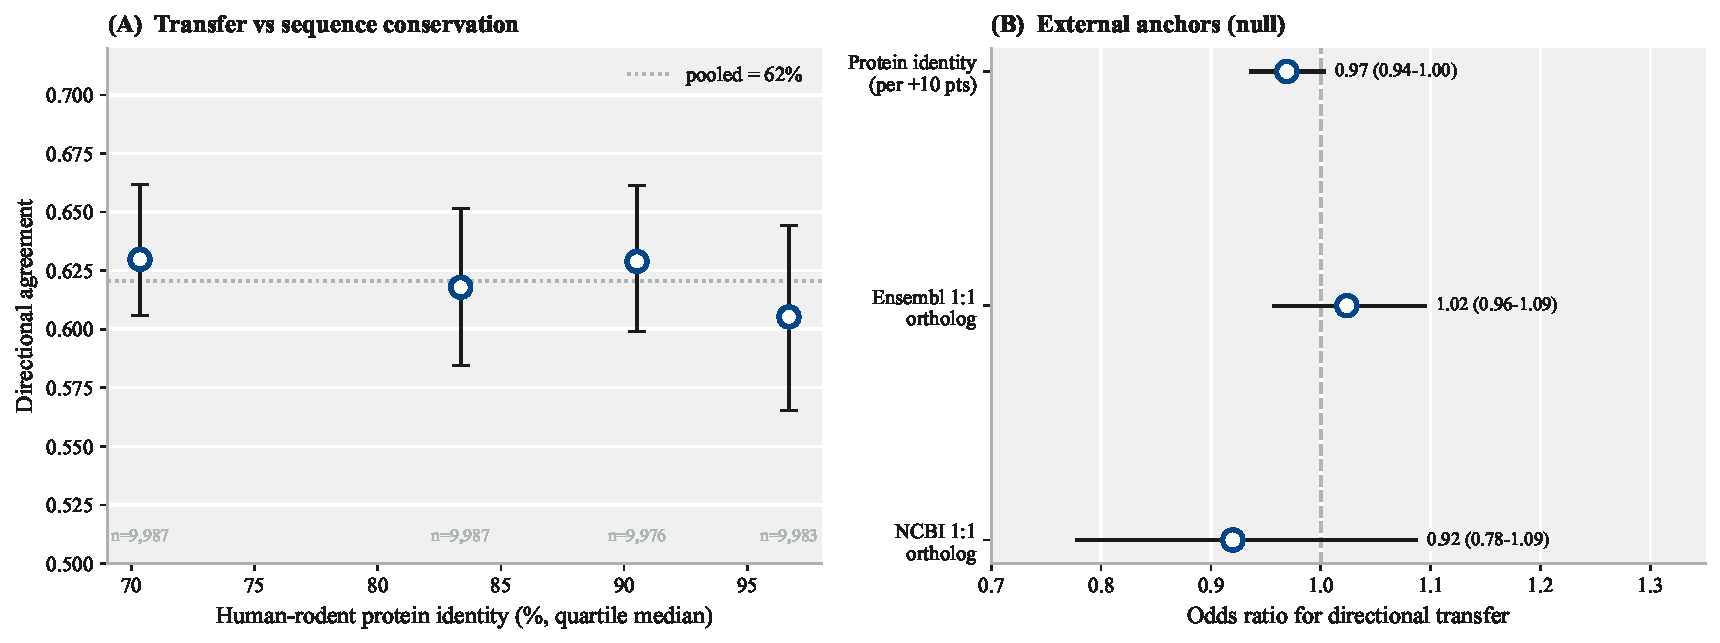
\includegraphics[width=\linewidth]{F6_conservation.pdf}
\caption{External conservation anchor (pre-registered). (A) Independent
directional agreement by quartile of human-rodent protein identity, with
cluster-bootstrap 95\% intervals; agreement is flat across the full identity
range. (B) Odds ratios for transfer from graded identity and from one-to-one
orthology (Ensembl and NCBI); all straddle 1. Sequence conservation is not
associated with directional transfer.}
\label{fig:6}
\end{figure}

\subsection{A catalogue of independent cross-species conflicts}

The independence guard also yields a practical by-product: effects that are
independently and repeatedly curated in opposite directions in humans and
rodents. These are candidate true species divergences or curation errors worth
targeted review, and they are enriched for well-studied environmental chemicals
(for example bisphenol A, dioxin and paraquat) acting on stress-response and
ribosomal genes. The full catalogue is provided in Supplementary Table~S9.

%=========================================================================
\section{Discussion}
%=========================================================================

Using more than a million curated chemical-gene effects, we find that when a
chemical's directional effect on a gene is established independently in rodents,
it holds in humans about three fifths of the time, only modestly above chance
and barely better than one rodent predicts another. The result is easy to
misread in either direction, and the guardrails matter. Without an independence
guard the same data yield 89\% agreement, a number that would license
comfortable extrapolation and is almost entirely an artefact of the same
publication being curated into both species. With the guard, and against a
within-rodent benchmark, the honest picture emerges: cross-species disagreement
among curated directional chemical-gene effects looks far more like a problem of
reproducibility and context dependence than a problem of phylogenetic distance.
We are careful to state this as a claim about curated directional concordance,
not about controlled biological reproducibility, which our data cannot measure
directly.

Three findings support that reading and each is, we think, individually
useful. First, the disagreement is largely generic rather than human-specific:
the excess disagreement incurred by crossing from rodent to human, beyond that
incurred by crossing between two rodents, is not distinguishable from zero, and a
large share of disagreement is simply that a single species does not reproduce
its own directional call. Second, what transfers is governed by \emph{what is
measured} and \emph{how well it is established}, not by the kind of chemical.
Functional endpoints such as enzyme activity and secretion transfer well; bulk
expression is mediocre and DNA methylation is uninformative; and any effect
replicated across a handful of studies transfers nearly deterministically. Third,
an external and pre-registered axis of molecular similarity, protein sequence
conservation, was not associated with transfer. We are cautious about causal
language, but this is the pattern expected if diverged proteins were not the main
driver: had the barrier been largely about sequence divergence, conservation
should have tracked agreement, and it did not. The finding sits comfortably
beside long-standing scepticism about the ortholog conjecture, the assumption
that orthologous genes retain equivalent function across species
\citep{nehrt2011,chen2012ortholog}.

For practice, the actionable content is specific. A rodent directional call on a
functional endpoint, or one supported by several independent studies, is a
reasonable basis for a human expectation; a single-study call on expression or
methylation is not. Because transferability localises to the specific
chemical-gene pair and cannot be recovered from chemical class or from broad
gene properties, screening strategies that triage chemicals by class, or that
lean on sequence conservation to argue for cross-species relevance, are weakly
grounded for directional prediction. These conclusions bear directly on the new
approach methodologies agenda \citep{wu2026science,marshall2023}:
they argue for weighting evidence by endpoint type and replication rather than by
taxonomic proximity, and they supply a quantitative baseline against which
human-relevant assays can be judged.

The work also carries a general methodological warning for anyone mining curated
biomedical databases for cross-species or cross-context concordance. When two
facts are curated from a shared literature, their agreement is not evidence; it
is bookkeeping. The 27-point gap between guarded and unguarded estimates here is
a concrete measure of how badly that can mislead, and the same guard, disjoint
supporting references, is applicable to any database that records provenance.

\subsection{Limitations}

The most important limitation is intrinsic to the substrate and to the estimand.
CTD is curated from published findings, so what we measure is agreement between
curated directional calls, not a controlled biological replication: a matched
human and rodent call may come from different tissues, doses, exposure durations
or cell types. Our estimates are therefore literature-level directional
concordance, a necessary condition for biological reproducibility rather than a
direct measurement of it, and every estimand is conditional on curation and
inherits publication and curation bias, with effects measured in both species
enriched for well-studied, ``interesting'' genes. This constraint cannot be
removed by any CTD-only analysis, which is precisely why we anchored the study to
an external axis; that the anchor returned a null strengthens rather than weakens
the reproducibility reading, but it does not convert the design into an
experimental one. Within-species ``inconsistency'' conflates genuine context
dependence, real tissue, dose and time effects, with curation noise, and our data
cannot fully separate them. The mouse-versus-rat benchmark is likewise not a pure
noise floor: mouse and rat are distinct species, so it blends curation
reproducibility with genuine mouse-rat biological divergence. Because it absorbs
some real divergence, it slightly overstates the achievable reproducibility and
so makes our estimate of the human-versus-rodent excess conservative rather than
inflated. The pooling of mouse and rat into a single rodent group, while
appropriate for the primary translational question, could mask species-specific
patterns, although the mouse-versus-rat analysis argues against large ones. The
predictive ceiling we report is a statement about compact, prediction-time
features and does not exclude that richer molecular descriptors, unavailable
here, would do better. Finally, our conservation anchor is protein sequence
identity and one-to-one orthology; conservation of regulatory context or of
expression, which we did not measure, could in principle behave differently,
though there is no obvious mechanism by which it would rescue directional
transfer with which sequence conservation was not associated.

%=========================================================================
\section{Conclusions}
%=========================================================================

Independent directional agreement between rodent and human chemical-gene effects
is modest, is inflated roughly to 90\% by shared-publication co-curation if the
independence guard is dropped, and is barely above the agreement achievable
between two rodents. Transfer is governed by molecular endpoint and replication
depth rather than by chemical class, localises to the specific chemical-gene
pair, is only weakly predictable for unseen chemicals, and is not associated with
protein sequence conservation. Cross-species concordance of curated directional
chemical-gene effects is better described as a problem of reproducibility and
context dependence than of phylogenetic distance, and evidence should be weighted
by what was measured and how firmly it was established, not by taxonomic
proximity or sequence similarity. Because our estimands are literature-level
directional concordance conditional on curation, they bound rather than directly
measure biological reproducibility.

%=========================================================================
\section*{CRediT authorship contribution statement}
%=========================================================================

The CRediT author contribution statement is provided on the separate title page
to preserve double-blind review.

\section*{Declaration of competing interest}
The authors declare that they have no known competing financial interests or
personal relationships that could have appeared to influence the work reported
in this paper.

\section*{Funding}
This research did not receive any specific grant from funding agencies in the
public, commercial, or not-for-profit sectors.

\section*{Data availability}
The Comparative Toxicogenomics Database is openly available at
\url{https://ctdbase.org}; NCBI \texttt{gene\_orthologs} and Ensembl Compara are
openly available from their respective providers. All analysis code and the
non-identifiable aggregate tables and figures supporting this study are openly
available at
\url{https://github.com/january-msemakweli/Cross-Species-Directional-Transfer-Chemical-Gene-Effects}
(and the corresponding Zenodo archive linked from that repository's Releases).
No restricted or patient-level data were used.

\section*{Declaration of generative AI and AI-assisted technologies in the
manuscript preparation process}
During the preparation of this work the authors used Grammarly AI in order to
improve the language and readability of the manuscript. After using this tool,
the authors reviewed and edited the content as needed and take full
responsibility for the content of the published article.

\section*{Acknowledgements}
The authors thank the curators and maintainers of the Comparative Toxicogenomics
Database, NCBI and Ensembl for the openly available resources that made this
work possible.

\clearpage

\begin{thebibliography}{99}
\expandafter\ifx\csname url\endcsname\relax
  \def\url#1{\texttt{#1}}\fi
\expandafter\ifx\csname urlprefix\endcsname\relax\def\urlprefix{URL }\fi
\expandafter\ifx\csname href\endcsname\relax
  \def\href#1#2{#2} \def\path#1{#1}\fi

\bibitem[Austine-Orimoloye et al.(2025)]{austine2025ensembl}
Austine-Orimoloye, O., Azov, A.G., Barba, M., Barnes, I., Becker, A., Boddu, S.,
et al., 2025. Ensembl 2025. Nucleic Acids Res. 53 (D1), D948-D957.
https://doi.org/10.1093/nar/gkae1071.

\bibitem[Brown et al.(2015)]{brown2015ncbigene}
Brown, G.R., Hem, V., Katz, K.S., Ovetsky, M., Wallin, C., Ermolaeva, O., et
al., 2015. Gene: a gene-centered information resource at NCBI. Nucleic Acids Res.
43 (D1), D36-D42. https://doi.org/10.1093/nar/gku1055.

\bibitem[Chen and Zhang(2012)]{chen2012ortholog}
Chen, X., Zhang, J., 2012. The ortholog conjecture is untestable by the current
gene ontology but is supported by RNA sequencing data. PLoS Comput. Biol. 8 (11),
e1002784. https://doi.org/10.1371/journal.pcbi.1002784.

\bibitem[Clark and Steger-Hartmann(2018)]{clark2018}
Clark, M., Steger-Hartmann, T., 2018. A big data approach to the concordance of
the toxicity of pharmaceuticals in animals and humans. Regul. Toxicol.
Pharmacol. 96, 94-105. https://doi.org/10.1016/j.yrtph.2018.04.018.

\bibitem[Davis et al.(2025)]{davis2025ctd}
Davis, A.P., Wiegers, T.C., Sciaky, D., Barkalow, F., Strong, M., Wyatt, B., et
al., 2025. Comparative Toxicogenomics Database's 20th anniversary: update 2025.
Nucleic Acids Res. 53 (D1), D1328-D1334. https://doi.org/10.1093/nar/gkae883.

\bibitem[Davison and Hinkley(1997)]{davison1997boot}
Davison, A.C., Hinkley, D.V., 1997. Bootstrap Methods and Their Application.
Cambridge University Press, Cambridge.

\bibitem[Friedman(2001)]{friedman2001gbm}
Friedman, J.H., 2001. Greedy function approximation: a gradient boosting machine.
Ann. Stat. 29 (5), 1189-1232. https://doi.org/10.1214/aos/1013203451.

\bibitem[Kaufman et al.(2012)]{kaufman2012leakage}
Kaufman, S., Rosset, S., Perlich, C., Stitelman, O., 2012. Leakage in data
mining: formulation, detection, and avoidance. ACM Trans. Knowl. Discov. Data 6
(4), 15. https://doi.org/10.1145/2382577.2382579.

\bibitem[Ke et al.(2017)]{ke2017lightgbm}
Ke, G., Meng, Q., Finley, T., Wang, T., Chen, W., Ma, W., et al., 2017. LightGBM:
a highly efficient gradient boosting decision tree. Adv. Neural Inf. Process.
Syst. 30, 3146-3154.

\bibitem[Leenaars et al.(2019)]{leenaars2019}
Leenaars, C.H.C., Kouwenaar, C., Stafleu, F.R., Bleich, A., Ritskes-Hoitinga, M.,
De Vries, R.B.M., et al., 2019. Animal to human translation: a systematic
scoping review of reported concordance rates. J. Transl. Med. 17 (1), 223.
https://doi.org/10.1186/s12967-019-1976-2.

\bibitem[Liu and Fan(2026)]{liu2026}
Liu, X., Fan, F., 2026. A large-scale concordance study of toxicity findings
across preclinical species and humans for small molecules and biologics. Front.
Toxicol. 8, 1731947. https://doi.org/10.3389/ftox.2026.1731947.

\bibitem[Marshall et al.(2023)]{marshall2023}
Marshall, L.J., Bailey, J., Cassotta, M., Herrmann, K., Pistollato, F., 2023.
Poor translatability of biomedical research using animals: a narrative review.
Altern. Lab. Anim. 51 (2), 102-135.

\bibitem[Mattingly et al.(2003)]{mattingly2003ctd}
Mattingly, C.J., Colby, G.T., Forrest, J.N., Boyer, J.L., 2003. The Comparative
Toxicogenomics Database (CTD). Environ. Health Perspect. 111 (6), 793-795.

\bibitem[Nehrt et al.(2011)]{nehrt2011}
Nehrt, N.L., Clark, W.T., Radivojac, P., Hahn, M.W., 2011. Testing the ortholog
conjecture with comparative functional genomic data from mammals. PLoS Comput.
Biol. 7 (6), e1002073. https://doi.org/10.1371/journal.pcbi.1002073.

\bibitem[Pedregosa et al.(2011)]{pedregosa2011sklearn}
Pedregosa, F., Varoquaux, G., Gramfort, A., Michel, V., Thirion, B., Grisel, O.,
et al., 2011. Scikit-learn: machine learning in Python. J. Mach. Learn. Res. 12,
2825-2830.

\bibitem[Russell and Burch(1959)]{russell1959}
Russell, W.M.S., Burch, R.L., 1959. The Principles of Humane Experimental
Technique. Methuen, London.

\bibitem[Seok et al.(2013)]{seok2013}
Seok, J., Warren, H.S., Cuenca, A.G., Mindrinos, M.N., Baker, H.V., Xu, W., et
al., 2013. Genomic responses in mouse models poorly mimic human inflammatory
diseases. Proc. Natl. Acad. Sci. USA 110 (9), 3507-3512.
https://doi.org/10.1073/pnas.1222878110.

\bibitem[Shrout and Fleiss(1979)]{shrout1979icc}
Shrout, P.E., Fleiss, J.L., 1979. Intraclass correlations: uses in assessing
rater reliability. Psychol. Bull. 86 (2), 420-428.
https://doi.org/10.1037/0033-2909.86.2.420.

\bibitem[Takao and Miyakawa(2015)]{takao2015}
Takao, K., Miyakawa, T., 2015. Genomic responses in mouse models greatly mimic
human inflammatory diseases. Proc. Natl. Acad. Sci. USA 112 (4), 1167-1172.
https://doi.org/10.1073/pnas.1401965111.

\bibitem[Wilson(1927)]{wilson1927}
Wilson, E.B., 1927. Probable inference, the law of succession, and statistical
inference. J. Am. Stat. Assoc. 22 (158), 209-212.
https://doi.org/10.1080/01621459.1927.10502953.

\bibitem[Wu et al.(2026)]{wu2026science}
Wu, X., Wu, M.A., Zou, J., Kleinstreuer, N., Wu, J.C., 2026. Reimagining
human-centric drug development with new approach methodologies. Science 392
(6796), 371-378.

\end{thebibliography}

\end{document}
